

Los archivos por lotes (Batch o Script Shell) \cite{Silberschatz1999} son
 aquellos que contienen instrucciones para el sistema operativo en formato
 ASCII por lo que son dependientes de \'el, por lo general tienen la extensi\'on
 .bat o .sh, sin embargo, para el caso de UNIX esto no es obligatorio. En la
 figura~\ref{fig:script} se muestra el c\'odigo de un archivo por lotes y la 
 ejecuci\'on en consola.



\begin{figure}[h]
\centering
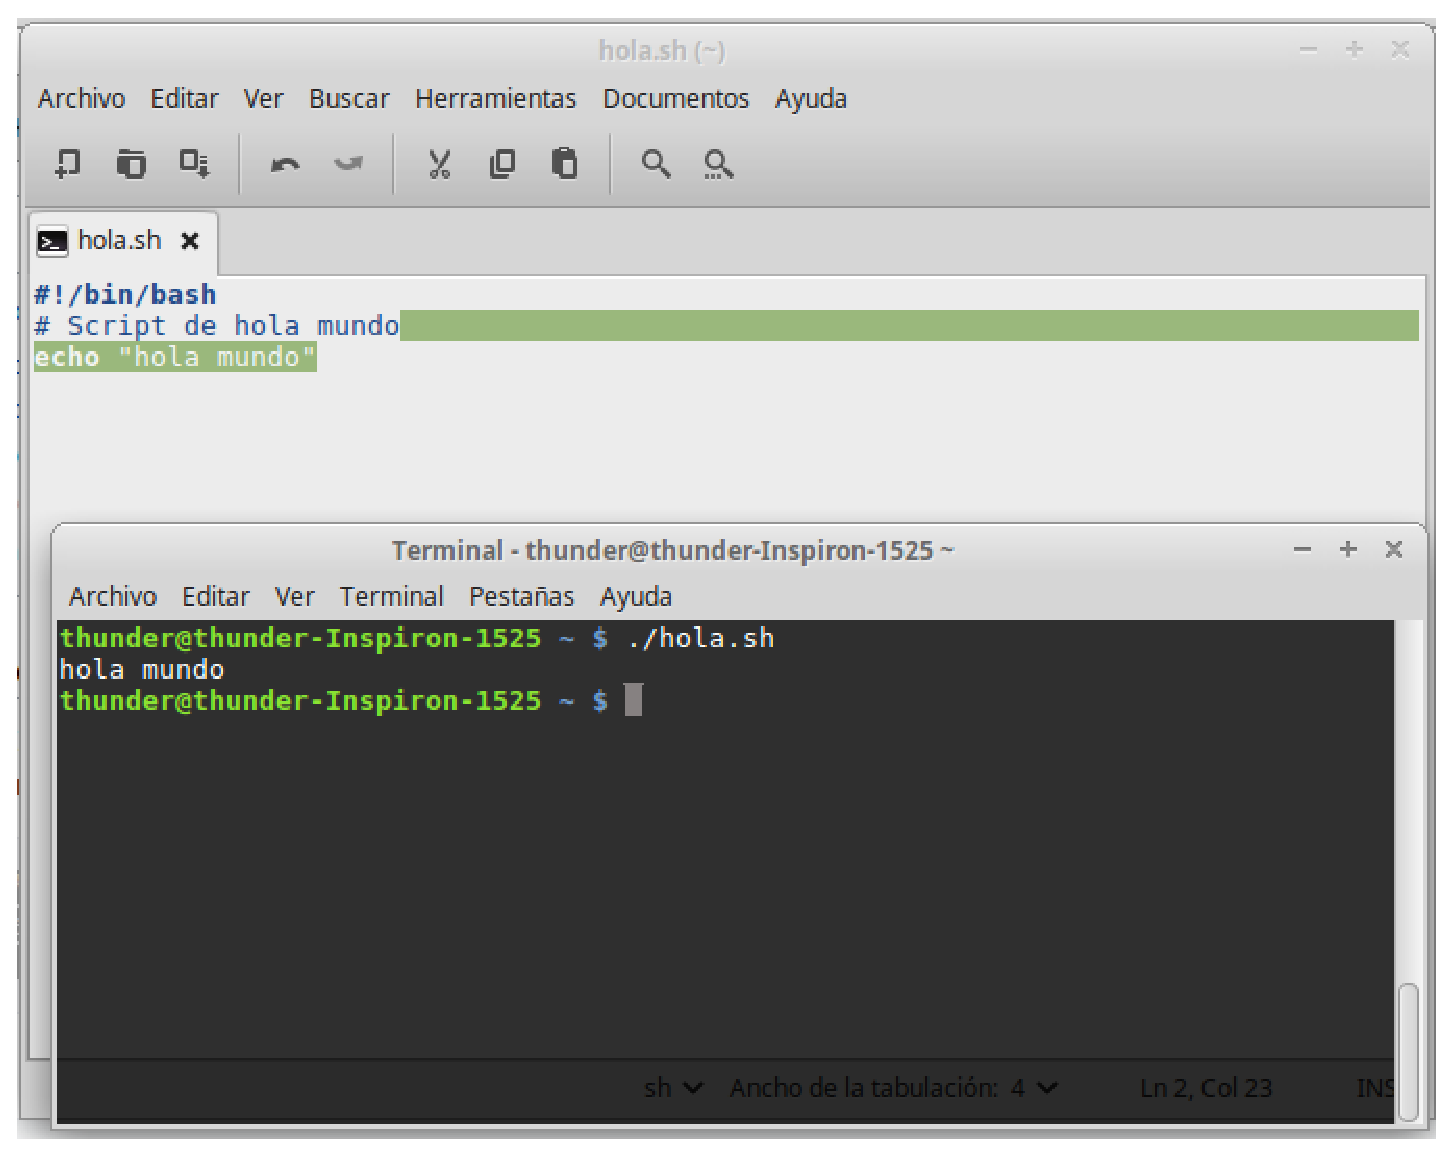
\includegraphics[width=0.7\columnwidth]{chap2/Imagenes/Script.eps}
\caption{Ejecuci\'on de un archivo por lotes en Linux.}
\label{fig:script}
\end{figure}